\documentclass[a4paper, 11pt]{article}
\usepackage[czech]{babel}
\usepackage[utf8x]{inputenc}
\usepackage[IL2]{fontenc}
\usepackage{times}
\usepackage[left=2cm, top=3cm, text={17cm, 24cm}]{geometry}
\usepackage[unicode]{hyperref}

\usepackage{Tabbing}
\usepackage{multirow}
\usepackage[noline,ruled,linesnumbered,czech]{algorithm2e}
\usepackage{graphicx}
\usepackage{epstopdf}


\begin{document}
\catcode`\-=12
\thispagestyle{empty}
\begin{center}
  {\Huge\textsc{Vysoké učení technické v~Brně \\ }}
  {\huge\textsc{Fakulta informačních technologií \\}}
  \vspace{\stretch{0.382}}
  {\LARGE{Typografie a publikování\,--\,3. projekt \\ }}
  {\Huge{Tabulky a obrázky \\}}
  \vspace{\stretch{0.618}}
  {\Large \today \hfill Tomáš Coufal}
\end{center}
\newpage
\setcounter{page}{1}

\section{Úvodní strana}
Název práce umístěte do zlatého řezu a nezapomeňte uvést dnešní datum a vaše jméno a příjmení.

\section{Tabulky}
Pro sázení tabulek můžeme použít buď prostření\texttt{ tabbing }nebo prostření\texttt{ tabular}.

\subsection{Prostředí{\texttt{ tabbing}}}
Při použití\texttt{ tabbing }vypadá tabulka následovně:
\begin{tabbing}
  \hspace{2.75cm} \= \hspace{1.25cm} \= \kill
  \bfseries Ovoce \> \bfseries Cena \> \bfseries Množství \\
  Jablka \> 25,90 \> 3\,kg \\
  Hrušky \> 27,40 \> 2,5\,kg \\
  Vodní melouny \> 35,-- \> 1\,kus \\
\end{tabbing}
Toto prostření se dá také použít pro sázení algoritmů, ovšem vhodnější je použít prostředí\texttt{ algorithm }nebo\texttt{ algorithm2e }(viz sekce \ref{sekce:3}).

\subsection{Prostředí{\texttt{ tabular}}}
Další možností, jak vytvořit tabulku, je použít prostředí\texttt{ tabular}. Tabulky pak budou vypadat takto\footnote{Kdyby byl problém s\texttt{ cline}, zkuste se podívat třeba sem: http://www.abclinuxu.cz/tex/poradna/show/325037.}.

\bigskip
\begin{table}[ht]
  \center
  \begin{tabular}{ |c|c|c| }
    \hline
    \multirow{3}{1cm}{\textbf{Měna}} & \multicolumn{2}{|c|}{\textbf{Cena}} \\
    \cline{2-3}
    & \textbf{nákup} & \textbf{prodej} \\
    \hline
    EUR & 27,34 & 27,42 \\
    GBP & 33,09 & 33,21 \\
    USD & 19,87 & 19,95 \\
    \hline
  \end{tabular}
  \caption{Tabulka kurzů k~dnešnímu dni}
  \label{tabulka:1}
\end{table}

\bigskip
\begin{table}[ht]
  \center
  \begin{tabular}{ |c|c| }
    \hline
    A~& $\lnot$A \\
    \hline
    P & N \\
    \hline
    O~& O~\\
    \hline
    X & X \\
    \hline
    N & P \\
    \hline
  \end{tabular}
  \begin{tabular}{ |c|c|c|c|c|c| }
    \hline
    \multicolumn{2}{|c|}{\multirow{2}{*}{A $\land$ B}} &\multicolumn{4}{|c|}{\emph{B}} \\
    \cline{3-6}
    \multicolumn{2}{|c|}{} & \textbf{P} & \textbf{O} & \textbf{X} & \textbf{N} \\
    \hline
    \multirow{4}{*}{A} & \textbf{P} & P & O~& X & N \\
                       & \textbf{O} & O~& O~& N & N \\
                       & \textbf{X} & X & N & X & N \\
                       & \textbf{N} & N & N & N & N \\
    \hline
  \end{tabular}
  \begin{tabular}{ |c|c|c|c|c|c| }
    \hline
    \multicolumn{2}{|c|}{\multirow{2}{*}{A $\lor$ B}} &\multicolumn{4}{|c|}{\emph{B}} \\
    \cline{3-6}
    \multicolumn{2}{|c|}{} & \textbf{P} & \textbf{O} & \textbf{X} & \textbf{N} \\
    \hline
    \multirow{4}{*}{A} & \textbf{P} & P & P & P & P \\
                       & \textbf{O} & P & O~& P & O~\\
                       & \textbf{X} & P & P & X & X \\
                       & \textbf{N} & P & O~& X & N \\
    \hline
  \end{tabular}
  \begin{tabular}{ |c|c|c|c|c|c| }
    \hline
    \multicolumn{2}{|c|}{\multirow{2}{*}{A $\to$ B}} &\multicolumn{4}{|c|}{\emph{B}} \\
    \cline{3-6}
    \multicolumn{2}{|c|}{} & \textbf{P} & \textbf{O} & \textbf{X} & \textbf{N} \\
    \hline
    \multirow{4}{*}{A} & \textbf{P} & P & O~& X & N \\
                       & \textbf{O} & P & O~& P & O~\\
                       & \textbf{X} & P & P & X & X \\
                       & \textbf{N} & P & P & P & P \\
    \hline
  \end{tabular}
  \caption{Protože Kleeneho trojhodnotová logika už je "zastaralá", uvádíme si zde příklad čtyřhodnotové logiky}
  \label{tabulka:2}
\end{table}

\section{Algoritmy}\label{sekce:3}
Pokud budeme chtít vysázet algoritmus, můžeme použít prostředí\texttt{ algorithm }\footnote{Pro nápovědu, jak zacházet s~prostředím\texttt{ algorithm }, můžeme zkusit tuhle stránku.\\ http://ftp.cstug.cz/pub/tex/CTAN/macros/latex/contrib/algorithms/algorithms.pdf.}nebo\texttt{ algorithm2e}\footnote{Pro\texttt{ algorithm2e }zase tuhle: http://ftp.cstug.cz/pub/tex/CTAN/macros/latex/contrib/algorithm2e/doc/algorithm2e.pdf}. Příklad použití prostředí\texttt{ algorithm2e }viz Algoritmus \ref{algoritmus:1}.

\begin{algorithm}[h]\label{algoritmus:1}
  \caption{\textsc{Fast}SLAM}
  \SetNlSty{}{}{:}
  \SetNlSkip{-1.25em}
  \SetInd{0.85em}{0.85em}
  \SetKwInput{Input}{Input}\SetKwInOut{Output}{Output}
  \SetKwFor{For}{for}{do}{{end for}}
  \SetKw{KwTo}{\textnormal{to}}
  \DontPrintSemicolon
  \Input{$(X_{t-1}, u_t, z_t)$}
  \Output{$X_t$}
  \Indp
  \BlankLine
  $\overline{X_t} = X_t = 0$\;
  \For{$k = 1$ \KwTo $M$}
  {
    $x_t^{[k]} = $ \emph{sample\_motion\_model} $(v_t,x_{t-1}^{[k]})$\;
    $w_t^{[k]} = $ \emph{measurement\_model} $(z_t,x_t^{[k]},m_{t-1})$\;
    $m_t^{[k]} = $ \emph{updated\_occupancy\_grid} $(z_t,x_t^{[k]},m_{t-1}^{[k]})$\;
    $\overline{X_t} = \overline{X_t} + \langle x_x^{[m]}, w_t^{[m]}\rangle $
  }
  \For{$k = 1$ \KwTo $M$}
  {
    draw $i$ with probability $\approx$ $w_t^{[i]}$\;
    add $\langle x_x^{[k]}, m_t^{[k]}\rangle $ \KwTo $X_t $\;
  }
  \KwRet{$X_t$}
\end{algorithm}

\section{Obrázky}
Do našich článků můžeme samozřejmě vkládat obrázky. Pokud je obrázkem fotografie, můžeme klidně použít bitmapový soubor. Pokud by to ale mělo být nějaké schéma nebo něco podobného, je dobrým zvykem takovýto obrázek vytvořit vektorově.

\begin{figure}[htb]
  \begin{center}
    \scalebox{0.4}{{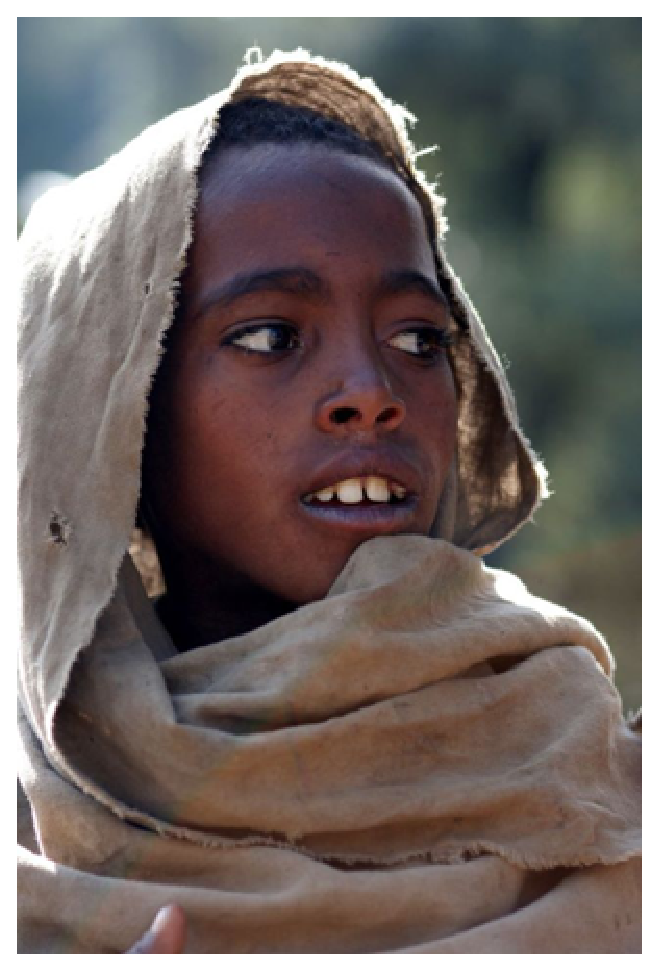
\includegraphics{etiopan.eps} }
    \reflectbox{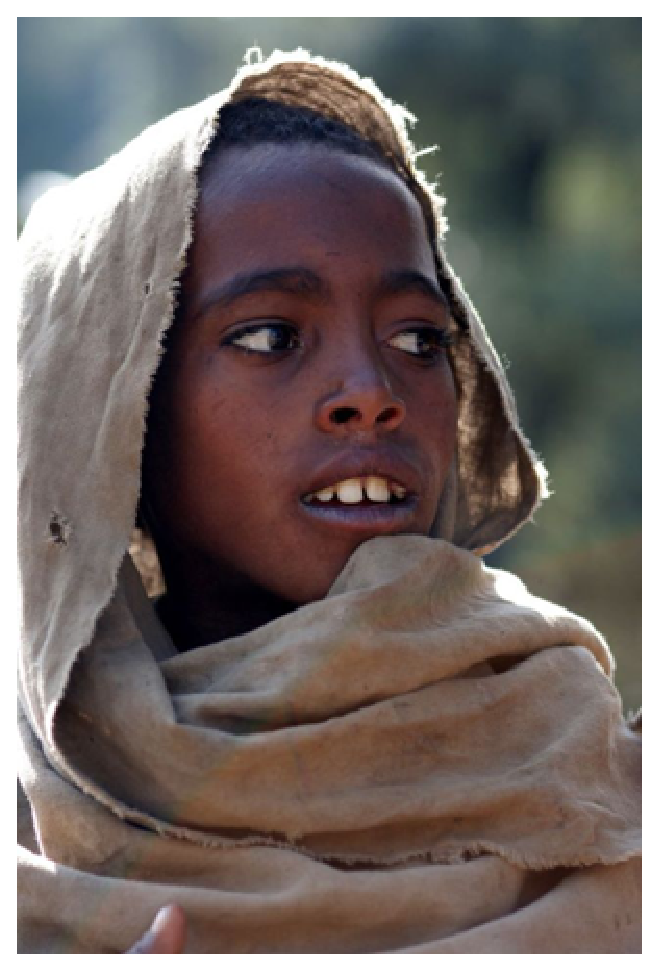
\includegraphics{etiopan.eps}}}
    \caption{Malý Etiopiánek a jeho bratříček}
    \label{obr:1}
  \end{center}
\end{figure}

\cleardoublepage
Rozdíl mezi vektorovým \dots
\begin{figure}[htb]
  \begin{center}
    \scalebox{0.4}{
\includegraphics{oniisan.eps} }
    \caption{Vektorový obrázek}
    \label{obr:2}
  \end{center}
\end{figure}

\noindent \dots a bitmapovým obrázkem
\begin{figure}[htb]
  \begin{center}
    \scalebox{0.6}{
\includegraphics{oniisan2.eps}}
    \caption{Bitmapový obrázek}
    \label{obr:3}
  \end{center}
\end{figure}

\noindent se projeví například při zvětšení.

Odkazy (nejen ty) na obrázky \ref{obr:1}, \ref{obr:2} a \ref{obr:3}, na tabulky \ref{tabulka:1} a \ref{tabulka:2} a také na algoritmus \ref{algoritmus:1} jsou udělány pomocí klíčových odkazů. Pak je ovšem potřeba zdrojový soubor přeložit dvakrát.

Vektorové obrázky lze vytvořit i přímo v~\LaTeX , například pomocí prostředí \texttt{picture}. Všechny rozměry jsou uváděny v~mm.

\newpage
\begin{figure}
  \setlength{\unitlength}{1,35mm}
  \setlength{\arrayrulewidth}{1pt}
  \begin{picture}(200,160)(-5,0)
    \linethickness{1pt}
    \put(0,0){\framebox(115,158.5){}}
    \multiput(15,0)(0,15){11}{\line(0,1){9}}
    \multiput(0,144)(15,0){8}{\line(2,0){10}}
    \put(30,124){\framebox(55,10){\textbf{Hlavička}}}
    \put(30,35){\framebox(55,75){\textbf{Textové tělo}}}
    \put(94,80){\framebox(15,10){\textbf{\shortstack{Okrajová \\ poznámka}}}}
    \put(30,10){\framebox(55,10){\textbf{Pata}}}
    \linethickness{0.3pt}
    \put(0,93){\vector(1,0){15}}\put(15,93){\vector(-1,0){15}}
    \put(85,93){\vector(1,0){9}}\put(94,93){\vector(-1,0){9}}
    \put(94,93){\vector(1,0){15}}\put(109,93){\vector(-1,0){15}}
    \put(30,137){\vector(1,0){55}}\put(85,137){\vector(-1,0){55}}
    \put(0,3){\vector(1,0){115}}\put(115,3){\vector(-1,0){115}}
    \put(112,0){\vector(0,1){158.5}}\put(112,158.5){\vector(0,-1){158.5}}
    \put(94,105){\vector(-1,-4){3}}
    \put(100,50){\vector(3,2){12}}
    \linethickness{0.2pt}
    \put(88,144){\vector(0,1){14.5}}
    \put(88,158.5){\vector(0,-1){14.5}}
    \put(88,134){\vector(0,1){10}}
    \put(88,144){\vector(0,-1){10}}
    \put(88,124){\vector(0,1){10}}
    \put(88,134){\vector(0,-1){10}}
    \put(88,110){\vector(0,1){14}}
    \put(88,124){\vector(0,-1){14}}
    \put(88,35){\vector(0,1){75}}
    \put(88,110){\vector(0,-1){75}}
    \put(88,20){\vector(0,1){15}}
    \put(88,35){\vector(0,-1){15}}
    \put(88,10){\vector(0,1){10}}
    \put(88,20){\vector(0,-1){10}}
    \put(95,154){Výška}
    \put(90,151){mezery = 14,5}
    \put(94,140){Výška}
    \put(90,137){mezery = 10}
    \put(94,130){Výška}
    \put(90,127){hlavičky = 10}
    \put(94,119){Výška}
    \put(90,116){mezery = 10}
    \put(91,106){Mezera = 9}
    \put(92,70){Výška}
    \put(90,67){těla = 75}
    \put(99,57){Výška}
    \put(94,53.5){stránky = 158,5}
    \put(94,30){Výška}
    \put(90,27){mezery = 15}
    \put(90,16){Výška}
    \put(90,13){paty = 10}
    \put(0.5,94.5){Mezera = 15}
    \put(97.5,97){Šířka}
    \put(95.5,94.5){boxu = 15}
    \put(48,138.5){Šířka boxu = 55}
    \put(48,4.5){Šířka stránky = 155}
  \end{picture}
  \caption{Vektorový obrázek v~prostředí {\texttt{picture}}}
\end{figure}
\end{document}
